\documentclass{article}
\usepackage[final,nonatbib]{neurips_2019}
\usepackage[utf8]{inputenc}
\usepackage[T1]{fontenc}
\usepackage{amsmath,amssymb,booktabs,graphicx,microtype,float}
\usepackage[hidelinks]{hyperref}
\hypersetup{pdftitle={Can Consistent Forces Recover Molecular Shapes?},pdfauthor={Shedrack Eze; Olufunke Abodunrin; Emmanuel Aaron; Muhammed Idris}}
\makeatletter
\renewcommand{\@noticestring}{11-785 Introduction to Deep Learning, Fall 2026. Group 9 midterm report, 23 October 2026.}
\makeatother
\title{Can Consistent Forces Recover Molecular Shapes?}
\author{Shedrack Eze (seze) \quad Olufunke Abodunrin (oabodunr)\\
\textbf{Emmanuel Aaron (eaaron) \quad Muhammed Idris (midris)}\\
Carnegie Mellon University \quad Group 9, Path 3}
\newcommand{\funit}{\mathrm{meV}/\text{\AA}}
\begin{document}
\maketitle
\begin{abstract}
Learned molecular forces describe pushes and pulls on atoms and can accelerate searches for stable molecular shapes, but accurate force predictions do not guarantee recovery of the correct shape. Three graph neural network formulations were evaluated on aspirin: forces calculated from negative energy slopes, forces predicted directly, and direct forces trained to agree with energy-derived forces. Consistency strength 0.1 achieved a validation force error of 38.024 meV/Å versus 38.186 for direct prediction, while requiring 1.985 times its CPU fitting-and-scoring time. All five tested model states, including the energy baseline, recovered zero of ten targets, although every target shape appeared in training. All 23 endpoints meeting the force stopping rule for direct and consistency models had atom groups separated beyond the model's 5 Å interaction range. Zero recovery prevents a ranking of methods; the diagnostics identify model and procedure limitations, while controlled movement-cap tests are needed to assess the effect of excessive atom movements.
\end{abstract}
\section{Introduction}
Repeated calculations of molecular energies and forces are expensive, so learned approximations can reduce simulation cost. Training changes a model's adjustable numbers, called parameters, to match reference examples.

Energy assigns a value to an atomic arrangement, like energy stored in a stretched spring whose pull points toward lower energy. Direct models predict force arrows; consistency training encourages agreement with negative energy slopes. Direct prediction skips the slope calculation and can be cheaper, but its forces need not follow one energy.

The objective is to compare correct-shape recovery at comparable force error, with computing cost measured separately. Recovery requires the search to reach its assigned target shape and meet the force stopping rule; neither condition alone establishes success.
\section{Literature Review}
Landscape17 supplies molecular shapes, reference forces and paths between stable arrangements~\cite{landscape}. It motivates checking final shapes beyond prediction errors, while Bigi et al. describe problems when direct forces do not follow one energy function~\cite{bigi}. Together, these studies motivate separating a force-based stop from structural success.

The models are built with E3x, software for networks that obey three-dimensional symmetry rules~\cite{e3x}. MACE supplies a separate established energy-derived model for predicting energies and forces~\cite{mace}. Earlier work already studies physical constraints in training losses~\cite{takamoto}. The unresolved question here is whether consistency improves recovery at comparable force error; consistency training itself is not new.

\section{Data and Preprocessing}
Each aspirin molecule has 21 atoms; Landscape17~\cite{landscape} reference energies and forces come from hybrid density-functional theory, an electron-physics calculation. These labels are calculated references rather than exact experimental truth.

A transition state is a high-energy arrangement with two downhill branches toward stable arrangements, called minima. A connection group contains both branches' records, which stay in the same partition to avoid separating the two sides of one transition state. Training adjusts parameters, validation selects settings and saved models, and the test partition is reserved for later trained-model evaluation.

The training set contains 26 connections and 4,891 records. Validation contains five connections and 974 records; testing contains six connections and 1,127 records. Training-only normalization puts energy and force errors on comparable scales, while shared minima mean that records are not independent examples of new destinations. Each branch targets the minimum it should reach; empirical classifications corrected 26 of 74 targets previously assigned from filename ordering. Earlier model-free software checks parsed test coordinates and labels but did not choose models or solver settings; no trained model has been scored on the test partition.
\section{Methodology}
\subsection{Model Architecture}
The E3x models are graph neural networks in which atoms are nodes and nearby atom pairs form links. Successive calculation stages, called layers, pass learned information along these links. Inputs are atom types and three-dimensional positions; outputs are one molecular energy and a force arrow for each atom. The three compared model types use 64 feature channels containing learned numbers and vectors, two message-passing rounds and eight radial functions describing pair distances.

Links extend to 5~\AA, where an angstrom (\AA) is $10^{-10}$ metres. Internal features carry scalar numbers and vectors with direction. Rotating a molecule rotates its predicted forces without changing its energy, properties called equivariance for forces and invariance for energy. The energy baseline has 43,521 parameters; models with separate energy and force outputs have 43,649.

The energy baseline calculates $\widehat{\mathbf F}^{E}=-\nabla_{\mathbf R}\widehat E$. Here, $\widehat E$ is predicted energy, $\mathbf R$ contains atom positions, and the gradient gives energy slopes along position coordinates. Both the direct and consistency models also predict energy trained against reference labels, so they are not force-only models. Ordinary direct training has no agreement penalty, while consistency training adds one. In this architecture, an isolated atom has zero direct force because it receives no directional message and its vector readout has no bias.
\subsection{Training and Evaluation}\label{sec:training}
The loss combines normalized squared energy error, normalized squared force error and, where applicable, force--energy disagreement; training adjusts parameters to reduce this number:
\begin{equation}
\mathcal L=w_E\,\mathrm{mean}(e_E^2)+w_F\,\mathrm{mean}(e_F^2)
+\lambda\,\mathrm{mean}\!\left[\left((\widehat{\mathbf F}^{D}-\widehat{\mathbf F}^{E})/s_F\right)^2\right].
\end{equation}
Normalized energy and force errors $e_E$ and $e_F$ use training scales $s_E\approx0.21584$~eV per molecule and $s_F\approx0.126886$~eV/\AA; $D$ denotes direct prediction. Supervised weights $w_E\approx0.01458$ and $w_F\approx1.985$ are rounded; configurations retain exact values. Energy training omits the agreement term; direct training uses $\lambda=0$, while consistency training uses positive $\lambda$.

Final E3x fits use Adam, an optimization method that updates parameters, with learning rate 0.003 and 64-bit floating-point arithmetic. Each update samples four records that can repeat, giving 800,000 sampled exposures across 200,000 updates. Two seeds specify random initialization and sampling, providing a limited repeatability check. E3x fits used an arm64 macOS CPU, Python 3.12.13, JAX/JAXlib 0.9.2 and E3x 1.0.2.

Validation occurs every 500 updates, including zero, and BEST is the first saved model state, or checkpoint, with minimum validation force error.

For each validation connection, force mean absolute error (MAE) averages absolute errors over records, atoms and coordinate components; the final score averages the five connections equally. A consistency model matches direct prediction when its two-seed mean-force-error gap is within 10\% of the smaller mean and within both seed spans. A seed span is maximum minus minimum.

A millielectronvolt (meV) is one thousandth of an electronvolt; meV/\AA\ measures force as energy per distance.

Recovery additionally requires maximum absolute predicted force component $\leq0.01$~eV/\AA\ and aligned structural RMSD $\leq0.05$~\AA. Root-mean-square deviation (RMSD) measures typical atom-position disagreement after rotation, translation and allowed atom-symmetry matching. Small predicted force is a stopping condition; it is not small prediction error.

The force-fit adequacy criterion requires validation MAE $\leq50$~meV/\AA, approximately 20\% below zero-force prediction. The recovery adequacy criterion requires the selected energy baseline to recover at least one branch and exceed the measured unchanged-start count. This checks whether the procedure improves the starting structures.

\subsection{Relaxation Procedure}
Adaptive force-following relaxation proposes $\mathbf R_{\mathrm{trial}}=\mathbf R+\eta\widehat{\mathbf F}$, where scale $\eta$ starts at 0.2~\AA$^2$/eV. A trial meeting the force stopping condition is accepted immediately. Otherwise, acceptance requires $\sum_{i,\alpha}\widehat F^{\mathrm{trial}}_{i\alpha}\widehat F^{\mathrm{current}}_{i\alpha}\geq-10^{-12}$~(eV/\AA)$^2$, summed over atoms $i$ and coordinate components $\alpha$.

The new force must not oppose the current force, apart from this numerical tolerance. Rejected trials halve the scale; accepted trials double it up to 1.0~\AA$^2$/eV. Each branch permits 1,500 force attempts, with no energy-decrease test or per-atom movement cap. FIRE and BFGS optimizers were not compared.

\section{Results and Discussion}
\subsection{Baseline Development}
Early E3x training on a 128-record subset plateaued, but MACE, which also derives forces from energy, fitted those records to 0.001515 of the zero-force squared error. Different settings prevent a controlled comparison, but the plateau did not establish an unavoidable data or energy-derived-force limit.

After 1,000 updates, energy and direct validation force MAEs worsened from 62.504 to 70.468 and 66.222~meV/\AA, respectively; both selected update zero as BEST.

Figure~\ref{fig:baseline} compares three 200,000-update energy baselines: A (width 32, learning rate 0.001), B (width 64, 0.003), and C (B with balanced loss weights). Width counts feature channels; A and B use equal normalized energy/force weights.

\begin{figure}[htbp]
\centering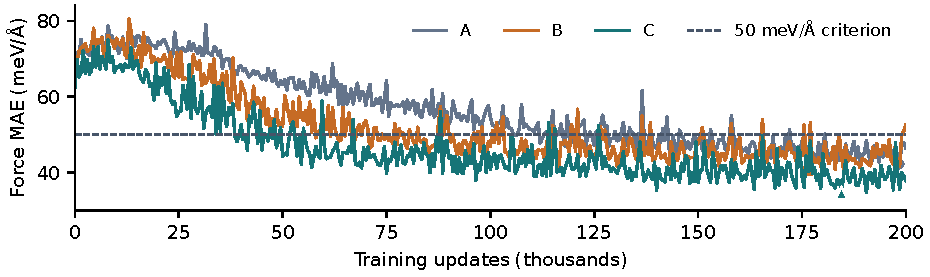
\includegraphics[width=0.85\linewidth]{figures/baseline-curves.pdf}
\caption{Energy-baseline validation, seed 0. The triangle marks C's BEST at update 184,500; the dashed line is the 50~meV/\AA\ force-fit adequacy criterion. Each point uses all 974 validation records, with equal connection weighting.}\label{fig:baseline}
\end{figure}

C's force MAE, 34.587~meV/\AA, passes the 50~meV/\AA\ force-fit adequacy criterion, outperforming B (40.370) and A (42.108). This improves on zero-force MAE, 62.504~meV/\AA, by 44.664\%. Energy MAE nevertheless rises from B's 28.178 to C's 126.990~meV per molecule. C's force-selected recipe was transferred without retuning despite this energy trade-off.
\subsection{Predictive Accuracy and Computational Cost}
C seed zero plus nine fits provided two seeds per row (Table~\ref{tab:prediction}). Consistency strength 0.1 reduces normalized force--energy disagreement squared error to 0.49--0.61, versus 116--379 for direct training. CPU fit-plus-score time is 1.985 times direct, excluding other diagnostics and overhead; this is not inference speed. Direct training has lower energy MAE, 76.684 versus 128.725~meV per molecule; the cause was not isolated.

\begin{table}[htbp]
\centering\small
\caption{Validation error at BEST. Force columns use meV/\AA; energy uses meV per molecule. Seed limits show two observed values, not confidence bounds.}\label{tab:prediction}
\begin{tabular}{lrrr}\toprule
Model & Mean force MAE & Seed min--max & Mean energy MAE\\\midrule
Energy-derived & 34.893 & 34.587--35.198 & 128.725\\
Direct & 38.186 & 37.291--39.082 & 76.684\\
Consistency $\lambda=0.1$ & 38.024 & 36.773--39.275 & 87.006\\
Consistency $\lambda=1$ & 34.683 & 33.723--35.643 & 112.341\\
Consistency $\lambda=10$ & 39.725 & 39.060--40.390 & 161.662\\\bottomrule
\end{tabular}
\end{table}

Only strength 0.1 meets the matching rule in Section~\ref{sec:training}.

BEST is optimistic because it selects among 401 checks. Over updates 150,000--200,000, the last 50,000 updates, baseline errors vary by 2.2--3.1~meV/\AA\ standard deviation across correlated checks. Nine subsequent fits finish 0.1--7.4~meV/\AA\ above BEST. The matching gap, 0.162~meV/\AA, is below this variation; matching does not establish equivalence.

MACE Run A independently scores 5.349~meV/\AA\ with equal connection weighting after 2,048 epochs on the same 4,891 training records. Each epoch uses 978 updates of five records, dropping the partial batch: 10,014,720 exposures overall, 12.52 times E3x's 800,000. Sampling, architecture, optimization and hardware differ; exposure alone does not explain the accuracy gap. This is an external reference, not a controlled efficiency comparison; MACE recovery remains unmeasured.

\subsection{Structural Recovery}
Five saved E3x checkpoints used adaptive force-following relaxation from ten shared branch starts across five validation connections. All six distinct branch-target minima appear in training. Unchanged starts recover zero targets, while all five checkpoints also recover 0/10 (Table~\ref{tab:recovery}). The energy baseline fails the recovery adequacy criterion; recovery cannot rank the methods.


\begin{table}[t]
\centering\small
\caption{All checkpoints recover 0/10 original targets. ``Wrong stop'' meets the predicted-force rule but misses the target shape. Reference-start controls begin at the six target minima; they are separate follow-up checks, called post-hoc analyses.}\label{tab:recovery}
\begin{tabular}{lrrr}\toprule
Checkpoint & Wrong stop & No convergence & Reference-start recovery\\\midrule
Energy C, seed 0 & 2 & 8 & 4/6\\
Direct, seed 0 & 4 & 6 & 1/6\\
Direct, seed 1 & 4 & 6 & 0/6\\
Consistency 0.1, seed 0 & 6 & 4 & 0/6\\
Consistency 0.1, seed 1 & 9 & 1 & 0/6\\\bottomrule
\end{tabular}
\end{table}

Across 50 model/branch outcomes, 25 stop with wrong geometry and 25 fail to converge. Reusing the same five connections does not create 50 independent paths. The reference-start controls favour the energy checkpoint under this procedure, but do not isolate a consistency-penalty effect.
\subsection{Endpoint Diagnostics}
Every model exceeds the stopping force threshold at all 11 stored aspirin minima, which include the six targets; reference labels stay below 2.745~meV/\AA. The 155 evaluations cover five checkpoints, each evaluated at ten starts, ten endpoints and eleven minima; all 50 stopping flags were reproduced. This mismatch at exact reference shapes does not exclude nearby shapes meeting both tolerances.

All 23 force-converged direct/consistency endpoints contain atom groups separated beyond the 5~\AA\ interaction range, leaving the interaction graphs disconnected. These are not intact molecular shapes, although internal fragment forces can remain. Only seven endpoints have every atom isolated, where the direct-force output is exactly zero automatically; this does not establish a correct molecular minimum.

Fixed before replay, four cases used seed-0 direct, consistency-0.1 and energy on connection 18's positive branch, and energy on connection 13's positive branch. These post-hoc cases reproduced saved endpoints; they were not sampled and are not representative. Two separated, with largest accepted atom movements of approximately 437~\AA\ for direct prediction and 268~\AA\ for energy-derived forces. The other two remained connected, with maxima approximately 0.086~\AA\ for consistency and 0.0061~\AA\ for energy-derived forces. The separated energy trace ended without convergence; both force-converged energy endpoints remained connected.

\subsection{Representation Study}
Feedback from a faculty member, a professor of materials science, suggested comparing models with and without rotation symmetry; all models here retain force rotation symmetry. E64 uses width-64 scalar/vector features; scalar S64 matches width and SP approximates parameter count. Their two-seed mean BEST force MAEs were 34.893, 39.542 and 41.358~meV/\AA, respectively, under E64-selected settings without scalar retuning. These preliminary findings await independent interpretation review and establish neither feature causality nor better recovery.

\section{Conclusion and Future Work}
Force-error matching did not deliver recovery under this procedure, and zero recovery cannot establish method equivalence.

\paragraph{Limitations.}
Evidence covers aspirin, five validation connections and two seeds, with shared minima. Validation selects settings and BEST; test generalization is unestablished. These checks do not isolate the procedure's contribution or establish real molecular break-up. Failed and incomplete trials remain recorded.

\paragraph{Changes from the proposal.}
Two seeds replace three, paracetamol is deferred until aspirin recovery is feasible, and revised adequacy criteria retain the small-subset failures; responsibilities changed and the representation check extends the proposal. Faculty suggested interactions beyond 7~\AA; the current 5~\AA\ range does not establish missing long-range interactions as the failure cause.
\paragraph{Planned Work.}
First, verify MACE predictions and run unchanged ten-start and six-reference controls. Then test a declared per-atom movement cap on the same checkpoints and starts, labelling reused-validation analysis post-hoc. Finally, compare prediction time and closed-loop work (summed force--displacement products around a loop) on identical hardware with declared matched-wall-time training budgets; smooth-energy work is zero apart from numerical integration error.
\paragraph{Team contributions and reproducibility.}
Shedrack completed data preparation, model/training integration and current MACE/E3x experiments. Olufunke authored the recovery evaluator. Emmanuel Aaron leads physical/cost analysis; Muhammed Idris leads MACE loading, prediction checks and independent reproduction.

{\raggedright Research code and evidence: GitHub, \href{https://github.com/Shedrackeze002/idl-molecular-force-consistency/tree/3fa5969e5a0c2fdeaebc76a05bace20799715203}{\nolinkurl{github.com/Shedrackeze002/idl-molecular-force-consistency}}, commit 3fa5969.\par}
\clearpage
\begin{thebibliography}{5}\small
\bibitem{landscape} V. C\u{a}rare et al. \href{https://doi.org/10.1038/s41524-025-01878-x}{Global properties of the energy landscape: a testing and training arena for machine learned potentials}. \emph{npj Computational Materials}, 12:9, 2026. doi:10.1038/s41524-025-01878-x.
\bibitem{bigi} F. Bigi, M. F. Langer and M. Ceriotti. \href{https://proceedings.mlr.press/v267/bigi25a.html}{The dark side of the forces: assessing non-conservative force models for atomistic machine learning}. \emph{ICML}, PMLR 267:4384--4414, 2025.
\bibitem{e3x} O. T. Unke and H. Maennel. \href{https://arxiv.org/abs/2401.07595}{E3x: E(3)-equivariant deep learning made easy}. arXiv:2401.07595, 2024.
\bibitem{mace} I. Batatia et al. \href{https://arxiv.org/abs/2206.07697}{MACE: Higher order equivariant message passing neural networks for fast and accurate force fields}. \emph{NeurIPS}, 35:11423--11436, 2022.
\bibitem{takamoto} M. Takamoto, V. Zaverkin and M. Niepert. \href{https://proceedings.mlr.press/v267/takamoto25a.html}{Physics-informed weakly supervised learning for interatomic potentials}. \emph{ICML}, PMLR 267:58282--58310, 2025.
\end{thebibliography}
\end{document}
